\begin{frame}{1.4 Transferência síncrona}
  Origem e destino usam um clock compartilhado ou um clock enviado junto com os dados.
  \begin{center}
  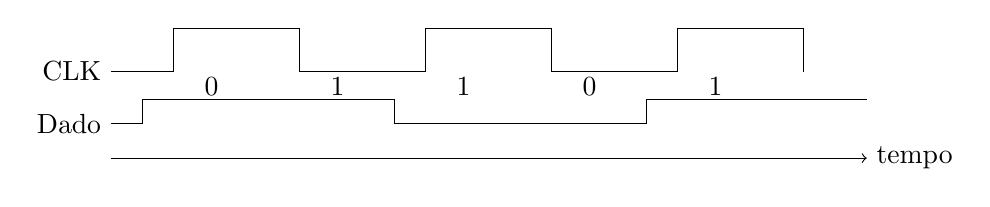
\begin{tikzpicture}[x=0.8cm,y=0.55cm]
    \draw[->] (0,0) -- (12,0) node[right]{tempo};
    \draw (0,2) node[left]{CLK} -- (1,2)--(1,3)--(3,3)--(3,2)--(5,2)--(5,3)--(7,3)--(7,2)--(9,2)--(9,3)--(11,3)--(11,2);
    \draw (0,0.8) node[left]{Dado} -- (0.5,0.8)--(0.5,1.35)--(4.5,1.35)--(4.5,0.8)--(8.5,0.8)--(8.5,1.35)--(12,1.35);
    \foreach \x/\v in {1.6/0,3.6/1,5.6/1,7.6/0,9.6/1} {\node at (\x,1.65) {\v};}
  \end{tikzpicture}
  \end{center}
  \begin{itemize}
    \item A leitura acontece em uma borda definida do clock.
    \item Comunicação simples e previsível em curtas distâncias.
    \item Exemplos: registradores, memória síncrona, SPI.
  \end{itemize}
\end{frame}